\documentclass{article}
\usepackage{CHEME-5660-Project}            % for camera-ready version
% \usepackage[review]{log_2022}  % for anonymous submission
% \usepackage[preprint]{log_2022}
%                                % for preprint version
% \usepackage[eatrack]{log_2022}
%                                % for accepted extended abstracts

\usepackage{booktabs}            % professional-quality tables
\usepackage{multirow}            % tabular cells spanning multiple rows
\usepackage{amsfonts}            % blackboard math symbols
\usepackage{graphicx}            % figures
\usepackage{duckuments}          % sample images

% If you want to use natbib:
\usepackage[numbers,compress,sort]{natbib}
%                                % for numerical citations
% \usepackage[sort,round]{natbib}
%                                % for textual citations

% If you want to use bibLaTeX, uncomment statements below:
% \usepackage[
%      backend=biber,
%      style=numeric-comp,
%      backref=true,
%      natbib=true]{biblatex}
% \addbibresource{reference.bib}

\title[CHEME 5660 Project, Fall 2022]{Your CHEME 5660 Project Title Goes Here. Make sure that the title is in Initial Caps --- The First Letter of Content Words Should be Made Capital Letters.}

\author[Y. Zhu et al.]{%
Yanqiao Zhu\thanks{Equal contribution.}\\
\institute{University of California, Los Angeles}\\
\email{yzhu@cs.ucla.edu}\And
Yuanqi Du\footnotemark[1]\\
\institute{Cornell University}\\
\email{yd392@cornell.edu}
}


\begin{document}

\maketitle

\begin{abstract}
Abstracts should be a single paragraph, ideally between 4--6 sentences long.
\end{abstract}

\section{Introduction}
Your project introduction goes here. 

\section{Materials and Methods}
Describe the materials and methods used in your study. This includes data, and approaches. 

\subsection{Subjections}
You can use different subsections if you want to.

\section{Results and Discussion}
Results and discussion goes here. Please use past tense for all results. We did this, we saw that. 


\section{Additional instructions. Delete me before submission}

\subsection{Author Information}
Author names are set in 10-point bold type, institution names and addresses are in 9-font, and email addresses are in 9-point typewriter font.
Each name should be centered above the corresponding institution and email address.
Authors can use \verb+\institute+ and \verb+\email+ to specify affiliations and email addresses respectively.

To ensure that the reference information in the bottom of the first page is rendered appropriately and concisely, 
please specify an abbreviated author list by shortening the first name of the first author in initials followed by 
``et al.'': \verb+\author[Y. Zhu et al.]{Yanqiao Zhu \and Yuanqi Du}+.

With the provided style file, the author information can be set in various styles.
If all authors are from the same institution, authors can use:
\begin{quote}
	\begin{verbatim}
		\author[F. Last et al.]
		 {First Last 1, First Last 2, ... \and First Last n \\
		  \institute{Institute \\ Address line}\\
		  \email{first.last@example.com}}
	\end{verbatim}
\end{quote}
For authors from different institutions, please use the \verb+\And+ command:
\begin{quote}
	\begin{verbatim}
		\author[F. Last et al.]
		 {First Last 1 \\
		  \institute{Institute 1\\ Address line} \\
		  \email{first.last.1@example.com}\And
		  First Last 2 \\
		  \institute{Institute 2\\ Address line} \\
		  \email{first.last.2@example.com}}
	\end{verbatim}
\end{quote}
If author names do not fit in one line, use the \verb+\AND+ command to start a separate row of authors:
\begin{quote}
	\begin{verbatim}
		\author[F. Last et al.]
		 {First Last 1, ..., \and First Last n \\
		  \institute{Institute 1\\ Address line} \\
		  \email{first.last.1@example.com}\AND
		  First Last n+1 \\
		  \institute{Institute 2\\ Address line} \\
		  \email{first.last.n.1@example.com}}
	\end{verbatim}
\end{quote}



\subsection{Headings and Sections}
All section headings should be numbered, flush left, and bold with content words capitalized.
\begin{itemize}
	\item First-level headings should be in 12-point type. Leave a 12-point space before and a 2-point space after the heading.
	\item Second-level headings should be in 10-point type. Leave a 8-point space before the heading and a 2-point space afterward.
	\item Third-level headings should be in 10-point type. Leave a 6-point space before and a 2-point space after the heading.
\end{itemize}
Please use no more than three levels of headings.

\paragraph{Paragraphs}
There is also a \verb+\paragraph+ command available, which sets the heading in bold, flush left, and inline with the text.
Leave a 6-point vertical space before the heading and 1em of horizontal space following the heading.

\paragraph{Footnotes}
Use footnotes to provide readers with additional information about a topic without interrupting the flow of the paper.
Footnotes should be numbered sequentially and placed in 9-point type at the bottom of the page on which they appear.
Precede the footnotes with a horizontal rule of 2 inches.
Note that footnotes should be properly typeset \emph{after} punctuation marks.\footnote{This is an example footnote.}

\subsection{Figures}
\begin{figure}
	\centering
	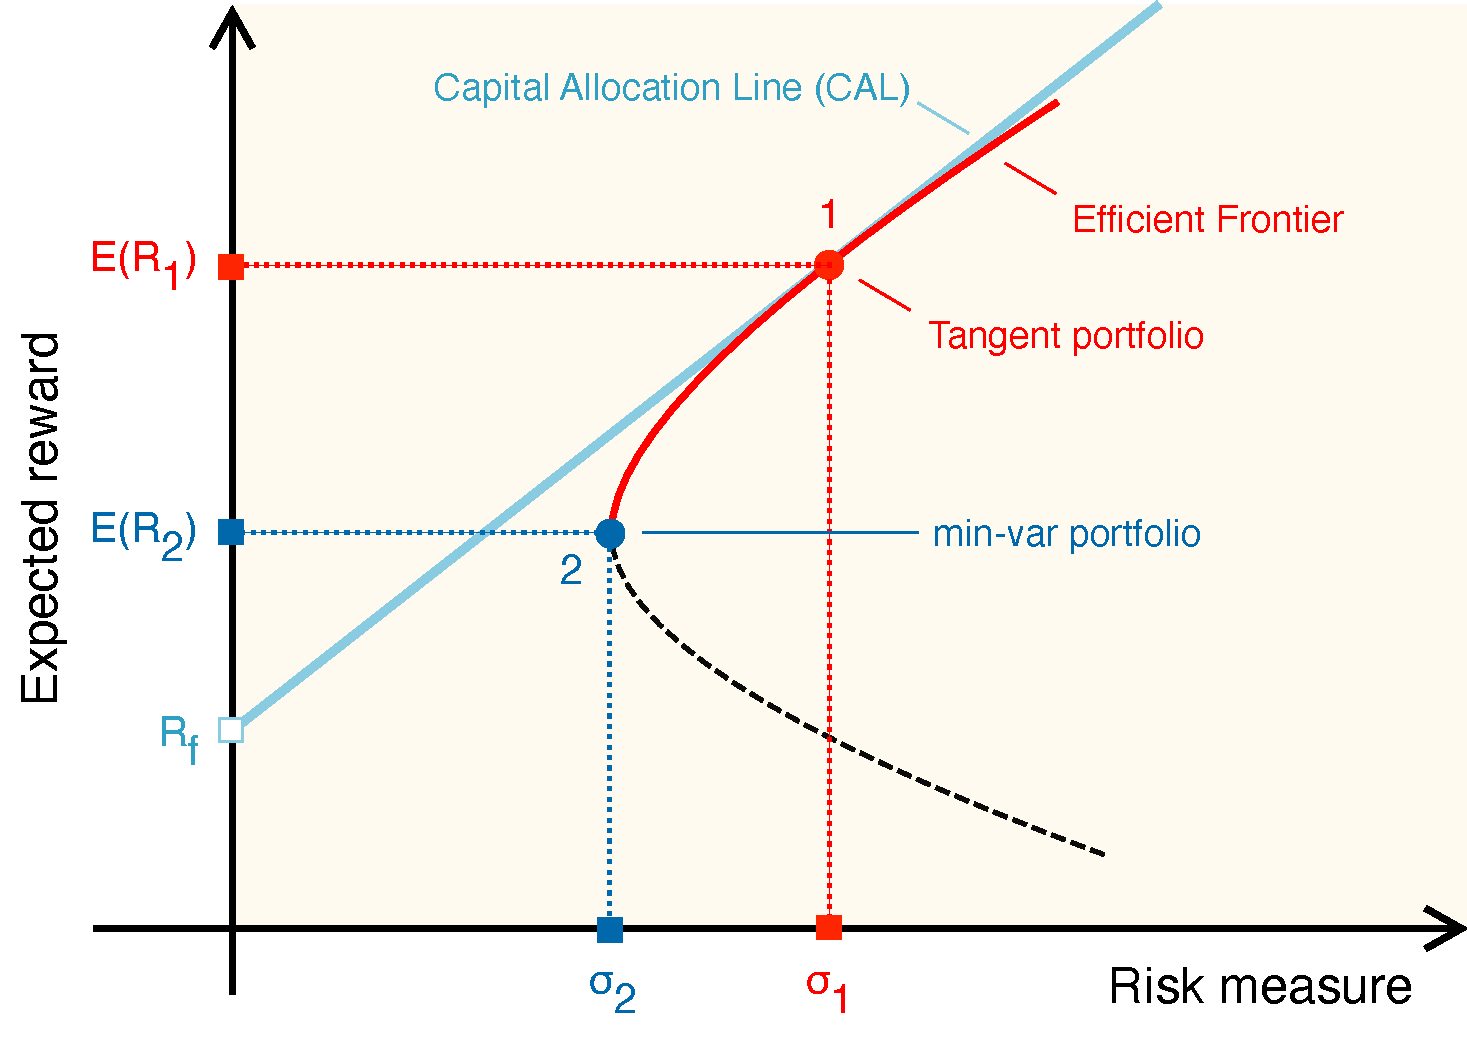
\includegraphics[width=0.5\linewidth]{./figs/Fig-Markowitz-Risk-Free-Asset-Example.pdf}
	\caption{A sample figure.}
	\label{fig:sample}
\end{figure}

All included artwork must be neat, legible, and separated from the text. You reference figures using thier label, see Figure~\ref{fig:sample} for an example.

\subsection{Tables}
\begin{table}
	\centering
	\caption{A sample table.}
	\label{tab:sample}
	\begin{tabular}{ccccc}
		\toprule
		\multirow{2.5}{*}{Method} & \multicolumn{2}{c}{Data 1} & \multicolumn{2}{c}{Data 2}  \\
		\cmidrule(lr){2-3} \cmidrule(lr){4-5}
		& \(\mathbf{X}\) & \(\mathbf{Y}\) & \(\mathbf{X}\) & \(\mathbf{Y}\) \\
		\midrule
		A & 0.8817  & 0.9572 & 0.1893 & 0.1725 \\
		B & 0.7126  & 0.2615 & 0.9173 & 0.1286 \\
		C & 0.2716  & 0.1826 & 0.2836 & 0.1836 \\
		\bottomrule
	\end{tabular}
\end{table}

Like figures, tables should be legible and numbered consecutively.
You reference tables using thier label, see Table~\ref{tab:sample} for an example.
We strongly suggest the use of the \texttt{booktabs} package (loaded by default) which provides the commands \verb+\toprule+, \verb+\midrule+, and \verb+\bottomrule+ to enhance the quality of tables.

\subsection{Paragraphs}
Paragraphs are separated by 1/2 line space (5.5 points).
Do not indent the first line of a given paragraph.

\subsection{Equations}
The provided style file loads the \verb+amsmath+ package automatically.
Unnumbered single-lined equations should be displayed using \verb+\[+ and \verb+\]+. For example:
\[
	\mathbf{X}' = \sigma(\widetilde{\mathbf{D}}^{-\frac{1}{2}}\widetilde{\mathbf{A}}\widetilde{\mathbf{D}}^{-\frac{1}{2}} \mathbf{XW}).
\]
Numbered single-line equations should be displayed using the \verb+equation+ environment. For example:
\begin{equation}
	\mathbf{X}' = \sigma(\widetilde{\mathbf{D}}^{-1}\widetilde{\mathbf{A}}\mathbf{XW}).
\end{equation}

\subsection{Bibliographies}
Use an unnumbered first-level heading for the references.
For a citation, use \verb+\cite+, e.g.,~\cite{Kipf:2017tc}.
For a textual citation, use \verb+\citet+, e.g.,~\citet{Velickovic:2018we}.
\emph{Any choice} of citation style is allowed as long as it is used consistently throughout the whole paper.
Additionally, both \verb+natbib+ and \verb+bibLaTeX+ packages are supported.
It is also possible to reduce the font size to \verb+\small+ (9-point font) when listing the references.

In the submission version, authors should refer to their own work in the third person for blind review.
In particular, avoid phrases that may reveal personal identities (e.g., ``in our earlier work~\cite{Hamilton:2017tp}, we have shown ...'').

\section*{Author Contributions}
Authors of accepted papers are \emph{encouraged} to include a statement that declares the individual contribution of every author, especially when there are co-authors that made equal contributions to the research.
You may adopt the \href{https://credit.niso.org/}{Contributor Roles Taxonomy (CRediT)} methodology for attributing contributions.
Do not include this section in the version for blind review.
This section does not count towards the page limit.

\section*{Acknowledgements}
The \LaTeX{} template for the CHEME-5660 project is heavily borrowed from LoG 2022 and NeurIPS 2022.

Do not include acknowledgements in the version for blind review.
If a paper is accepted, please place such acknowledgements in an unnumbered section at the end of the paper, immediately before the references.
The acknowledgements do not count towards the page limit.

% For natbib users:
\bibliographystyle{unsrtnat}
\bibliography{reference}
% For bibLaTeX users:
% \printbibliography

\appendix
\section{Appendix}
Any possible appendices should be placed after bibliographies.
If your paper has appendices, please submit the appendices together with the main body of the paper.
There will be no separate supplementary material submission.
The main text should be self-contained; reviewers are not obliged to look at the appendices when writing their review comments.

\end{document}
